
This paper presents the design and implementation of Dynamo, another highly available and scalable distributed data store built for Amazon’s platform. 

Using a relational database would lead to inefficiencies and limit scale and availability.

Dynamo uses a synthesis of well known techniques to achieve
scalability and availability: Data is partitioned and replicated
using consistent hashing [10], and consistency is facilitated by
object versioning [12]. The consistency among replicas during
updates is maintained by a quorum-like technique and a
decentralized replica synchronization protocol. 
Dynamo employs a gossip (reports about other people, typically involving details that are not confirmed as being true) based distributed failure detection and membership protocol. Dynamo is a completely decentralized system with
minimal need for manual administration. Storage nodes can be
added and removed from Dynamo without requiring any manual
partitioning or redistribution. 

\subsection{System Assumptions and Requirements}

\begin{description}
\item[Query Model] simple read and write operations to a data item that
is uniquely identified by a key. State is stored as binary objects
(i.e., blobs) identified by unique keys. No operations span
multiple data items and there is no need for relational schema. 

\item[ACID Properties] ACID (Atomicity, Consistency, Isolation,
Durability) is a set of properties that guarantee that database
transactions are processed reliably. In the context of databases, a
single logical operation on the data is called a transaction.
Experience at Amazon has shown that data stores that provide
ACID guarantees tend to have poor availability. Dynamo targets applications that operate with weaker consistency
(the “C” in ACID) if this results in high availability. Dynamo
does not provide any isolation guarantees and permits only single
key updates. 

\item[Efficiency] response within 300ms for 99.9\% of its requests for a
peak client load of 500 requests per second.

\item[Other Assumptions] Dynamo is used only by Amazon’s internal
services. Its operation environment is assumed to be non-hostile
and there are no security related requirements such as
authentication and authorization.
\end{description}

\subsection{Design considerations : Resolution on read, not write}
An important design consideration is to decide when to perform
the process of resolving update conflicts, i.e., whether conflicts
should be resolved during reads or writes. Many traditional data
stores execute conflict resolution during writes and keep the read
complexity simple [7]. In such systems, writes may be rejected if
the data store cannot reach all (or a majority of) the replicas at a
given time. On the other hand, Dynamo targets the design space
of an “always writeable” data store (i.e., a data store that is highly
available for writes). For a number of Amazon services, rejecting
customer updates could result in a poor customer experience. For
instance, the shopping cart service must allow customers to add
and remove items from their shopping cart even amidst network
and server failures. This requirement forces us to push the
complexity of conflict resolution to the reads in order to ensure
that writes are never rejected. 

The next design choice is who performs the process of conflict
resolution. This can be done by the data store or the application. If
conflict resolution is done by the data store, its choices are rather
limited. In such cases, the data store can only use simple policies,
such as “last write wins” [22], to resolve conflicting updates. On
the other hand, since the application is aware of the data schema it
can decide on the conflict resolution method that is best suited for
its client’s experience. For instance, the application that maintains
customer shopping carts can choose to “merge” the conflicting
versions and return a single unified shopping cart. Despite this
flexibility, some application developers may not want to write
their own conflict resolution mechanisms and choose to push it
down to the data store, which in turn chooses a simple policy such
as “last write wins”. 

\begin{description}
\item[Incremental scalability] Dynamo should be able to scale out one
storage host (henceforth, referred to as “node”) at a time, with
minimal impact on both operators of the system and the system
itself.

\item[Symmetry] Every node in Dynamo should have the same set of
responsibilities as its peers; there should be no distinguished node
or nodes that take special roles or extra set of responsibilities. In
our experience, symmetry simplifies the process of system
provisioning and maintenance

\item[Decentralization] An extension of symmetry, the design should
favor decentralized peer-to-peer techniques over centralized
control. In the past, centralized control has resulted in outages and
the goal is to avoid it as much as possible. This leads to a simpler,
more scalable, and more available system.

\item[Heterogeneity] The system needs to be able to exploit
heterogeneity in the infrastructure it runs on. e.g. the work
distribution must be proportional to the capabilities of the
individual servers. This is essential in adding new nodes with
higher capacity without having to upgrade all hosts at once.

\end{description}

\subsection{techniques used by Dynamo}

\begin{tabular}{p{4.5cm}|p{4.5cm}|p{4.5cm}}
Problem & Technique & Advantage \\
\hline
\hline
Partitioning & Consistent Hashing  & Incremental + Scalability \\
\hline
High Availability for writes  & Vector clocks with reconciliation during reads & Version size is decoupled from update rates. \\  
\hline
Handling temporary
failures  & Sloppy Quorum and
hinted handoff & Provides high
availability and
durability guarantee
when some of the
replicas are not
available.  \\
\hline
Recovering from
permanent failures & Anti-entropy using
Merkle trees & Synchronizes
divergent replicas in
the background. \\
\hline
Membership and
failure detection  & Gossip-based
membership protocol
and failure detection. & Preserves symmetry
and avoids having a
centralized registry
for storing
membership and
node liveness
information. \\
\hline 
\end{tabular}

Dynamo treats both the key and the object supplied by the caller
as an opaque array of bytes. It applies a MD5 hash on the key to
generate a 128-bit identifier, which is used to determine the
storage nodes that are responsible for serving the key. 

\subsubsection{Scale of hashing}

Each node in the
system is assigned a random value within this space which
represents its “position” on the ring. Each data item identified by
a key is assigned to a node by hashing the data item’s key to yield
its position on the ring, and then walking the ring clockwise to
find the first node with a position larger than the item’s position. 

Thus, each node becomes responsible for the region in the ring
between it and its predecessor node on the ring. The principle
advantage of consistent hashing is that departure or arrival of a
node only affects its immediate neighbors and other nodes remain
unaffected. 

Instead of mapping a node to a single point in the circle, each node gets
assigned to multiple points in the ring. To this end, Dynamo uses
the concept of “virtual nodes”. A virtual node looks like a single
node in the system, but each node can be responsible for more
than one virtual node. Effectively, when a new node is added to
the system, it is assigned multiple positions (henceforth, “tokens”)
in the ring. 

Advantage of this system :

\begin{itemize}
\item If a node becomes unavailable (due to failures or routine
maintenance), the load handled by this node is evenly
dispersed across the remaining available nodes. 
\item When a node becomes available again, or a new node is
added to the system, the newly available node accepts a
roughly equivalent amount of load from each of the other
available nodes. 
\item The number of virtual nodes that a node is responsible can
decided based on its capacity, accounting for heterogeneity
in the physical infrastructure.
\end{itemize}

\subsubsection{Replication}

To achieve high availability and durability, Dynamo replicates its
data on multiple hosts. Each data item is replicated at N hosts,
where N is a parameter configured “per-instance”. Each key, k, is
assigned to a coordinator node (described in the previous section).
The coordinator is in charge of the replication of the data items
that fall within its range. In addition to locally storing each key
within its range, the coordinator replicates these keys at the N-1
clockwise successor nodes in the ring. This results in a system
where each node is responsible for the region of the ring between
it and its Nth predecessor. In Figure 2, node B replicates the key k
at nodes C and D in addition to storing it locally. Node D will
store the keys that fall in the ranges (A, B], (B, C], and (C, D]. 

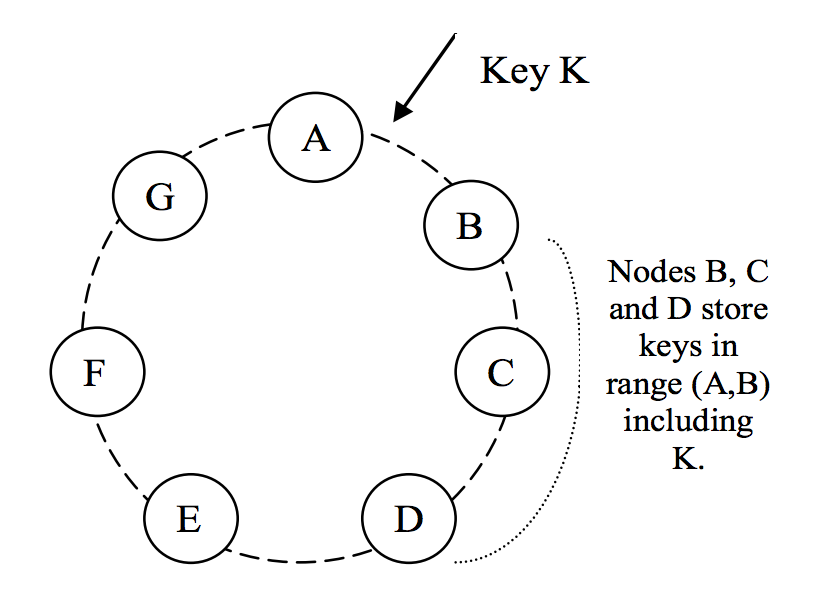
\includegraphics[width=0.5\linewidth]{img/dynamo.png}

The list of nodes that is responsible for storing a particular key is
called the preference list

\subsubsection{Data Versioning}

Dynamo provides eventual consistency, which allows for updates
to be propagated to all replicas asynchronously. 

Dynamo uses vector clocks [12] in order to capture causality
between different versions of the same object. A vector clock is
effectively a list of (node, counter) pairs. One vector clock is
associated with every version of every object. One can determine
whether two versions of an object are on parallel branches or have
a causal ordering, by examine their vector clocks. If the counters
on the first object’s clock are less-than-or-equal to all of the nodes
in the second clock, then the first is an ancestor of the second and
can be forgotten. Otherwise, the two changes are considered to be
in conflict and require reconciliation. 

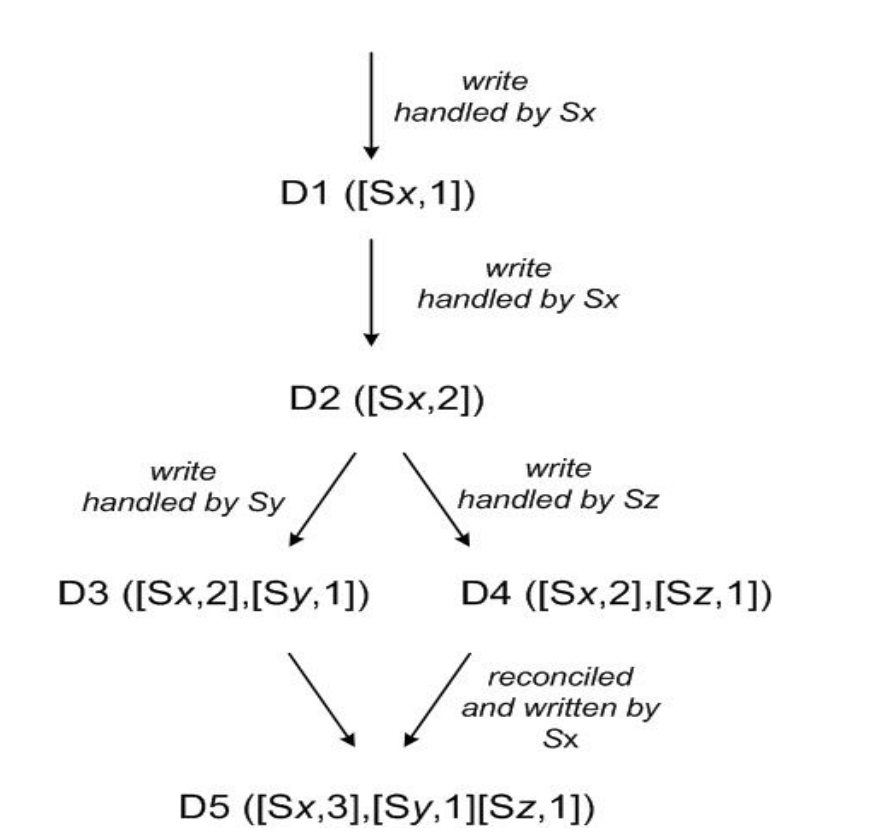
\includegraphics[width=0.5\linewidth]{img/vector_clocks.png}

In Dynamo, when a client wishes to update an object, it must
specify which version it is updating. This is done by passing the
context it obtained from an earlier read operation, which contains
the vector clock information. Upon processing a read request, if 
Dynamo has access to multiple branches that cannot be
syntactically reconciled, it will return all the objects at the leaves,
with the corresponding version information in the context. An
update using this context is considered to have reconciled the
divergent versions and the branches are collapsed into a single
new version.

It is desirable to limit the size of vector clock. To this
end, Dynamo employs the following clock truncation scheme:
Along with each (node, counter) pair, Dynamo stores a timestamp
that indicates the last time the node updated the data item. When
the number of (node, counter) pairs in the vector clock reaches a
threshold (say 10), the oldest pair is removed from the clock.
Clearly, this truncation scheme can lead to inefficiencies in
reconciliation as the descendant relationships cannot be derived
accurately. However, this problem has not surfaced in production
and therefore this issue has not been thoroughly investigated. 

\subsubsection{API interface}

get(K), put(K, X), put(K, C, X). K = key. X = content. C = context (for update).

To maintain consistency among its replicas, Dynamo uses a
consistency protocol similar to those used in quorum systems.
This protocol has two key configurable values: R and W. R is the
minimum number of nodes that must participate in a successful
read operation. W is the minimum number of nodes that must
participate in a successful write operation. Setting R and W such
that R + W > N yields a quorum-like system. In this model, the
latency of a get (or put) operation is dictated by the slowest of the
R (or W) replicas. For this reason, R and W are usually
configured to be less than N, to provide better latency. 

A node handling a read or write operation is known as the
coordinator. Typically, this is the first among the top N nodes in
the preference list. If the requests are received through a load
balancer, requests to access a key may be routed to any random
node in the ring. In this scenario, the node that receives the
request will not coordinate it if the node is not in the top N of the
requested key’s preference list. Instead, that node will forward the
request to the first among the top N nodes in the preference list. 

Upon receiving a put() request for a key, the coordinator generates
the vector clock for the new version and writes the new version
locally. The coordinator then sends the new version (along with the new vector clock) to the N highest-ranked reachable nodes. If
at least W-1 nodes respond then the write is considered
successful. 

Similarly, for a get() request, the coordinator requests all existing
versions of data for that key from the N highest-ranked reachable
nodes in the preference list for that key, and then waits for R
responses before returning the result to the client. If the
coordinator ends up gathering multiple versions of the data, it
returns all the versions it deems to be causally unrelated. The
divergent versions are then reconciled and the reconciled version
superseding the current versions is written back. 


\subsubsection{Handling Failures: Hinted Handoff}

It uses a “sloppy quorum”; all read and
write operations are performed on the first N healthy nodes from
the preference list, which may not always be the first N nodes
encountered while walking the consistent hashing ring. 

Consider the example of Dynamo configuration given in Figure 2
with N=3. In this example, if node A is temporarily down or
unreachable during a write operation then a replica that would
normally have lived on A will now be sent to node D. This is done
to maintain the desired availability and durability guarantees. The
replica sent to D will have a hint in its metadata that suggests
which node was the intended recipient of the replica (in this case
A). Nodes that receive hinted replicas will keep them in a
separate local database that is scanned periodically. Upon
detecting that A has recovered, D will attempt to deliver the
replica to A. Once the transfer succeeds, D may delete the object
from its local store without decreasing the total number of replicas
in the system. 

It is imperative that a highly available storage system be capable
of handling the failure of an entire data center(s). Data center
failures happen due to power outages, cooling failures, network
failures, and natural disasters. Dynamo is configured such that
each object is replicated across multiple data centers. In essence,
the preference list of a key is constructed such that the storage
nodes are spread across multiple data centers. These datacenters
are connected through high speed network links. This scheme of
replicating across multiple datacenters allows us to handle entire
data center failures without a data outage. 

\subsubsection{Handling permanent failures: Replica synchronization}

Hinted handoff works best if the system membership churn is low
and node failures are transient. There are scenarios under which
hinted replicas become unavailable before they can be returned to 
the original replica node. To handle this and other threats to
durability, Dynamo implements an anti-entropy (replica
synchronization) protocol to keep the replicas synchronized. 

To detect the inconsistencies between replicas faster and to
minimize the amount of transferred data, Dynamo uses Merkle
trees [13]. A Merkle tree is a hash tree where leaves are hashes of
the values of individual keys. Parent nodes higher in the tree are
hashes of their respective children. The principal advantage of
Merkle tree is that each branch of the tree can be checked
independently without requiring nodes to download the entire tree
or the entire data set. Moreover, Merkle trees help in reducing the
amount of data that needs to be transferred while checking for
inconsistencies among replicas. For instance, if the hash values of
the root of two trees are equal, then the values of the leaf nodes in
the tree are equal and the nodes require no synchronization. If not,
it implies that the values of some replicas are different. In such
cases, the nodes may exchange the hash values of children and the
process continues until it reaches the leaves of the trees, at which
point the hosts can identify the keys that are “out of sync”. Merkle
trees minimize the amount of data that needs to be transferred for
synchronization and reduce the number of disk reads performed
during the anti-entropy process.

Dynamo uses Merkle trees for anti-entropy as follows: Each node
maintains a separate Merkle tree for each key range (the set of
keys covered by a virtual node) it hosts. This allows nodes to
compare whether the keys within a key range are up-to-date. In
this scheme, two nodes exchange the root of the Merkle tree
corresponding to the key ranges that they host in common.
Subsequently, using the tree traversal scheme described above the
nodes determine if they have any differences and perform the
appropriate synchronization action. The disadvantage with this
scheme is that many key ranges change when a node joins or
leaves the system thereby requiring the tree(s) to be recalculated. 

\subsubsection{Ring Membership}
A node outage rarely signifies a permanent departure
and therefore should not result in rebalancing of the partition
assignment or repair of the unreachable replicas. Similarly,
manual error could result in the unintentional startup of new
Dynamo nodes. For these reasons, it was deemed appropriate to
use an explicit mechanism to initiate the addition and removal of
nodes from a Dynamo ring. An administrator uses a command
line tool or a browser to connect to a Dynamo node and issue a
membership change to join a node to a ring or remove a node
from a ring. 

\subsubsection{External Discovery}

To prevent logical
partitions, some Dynamo nodes play the role of seeds. Seeds are
nodes that are discovered via an external mechanism and are
known to all nodes. Because all nodes eventually reconcile their
membership with a seed, logical partitions are highly unlikely. 

\subsubsection{Failure Detection}

Dynamo used a decentralized failure detector to maintain a
globally consistent view of failure state. Later it was determined
that the explicit node join and leave methods obviates the need for
a global view of failure state. This is because nodes are notified of
permanent node additions and removals by the explicit node join
and leave methods and temporary node failures are detected by
the individual nodes when they fail to communicate with others
(while forwarding requests). 

\subsubsection{Implementation}
In Dynamo, each storage node has three main software
components: request coordination, membership and failure
detection, and a local persistence engine.

